\documentclass[12pt,a4paper]{book}
%\documentclass[a4paper,french]{book}
%\usepackage[17pt]{extsizes}


\input{../1ere-preambule}

\newcommand{\va}[1]{\lvert \ #1 \ \rvert}
\newcommand{\vaf}[1]{\left\lvert \ #1\  \right\rvert}

\begin{document}
\graphicspath{{images/}}
%\setcounter{chapter}{1}
\chapter[Fonction Affine - Exercices]{Fonction Affine et Linéaire \\ Exercices d'entrainement}
\thispagestyle{fancy}

\exerciceDS{}

Soit $f$ la fonction affine définie pour tout réel $x$ par $f(x)=5 x-4$.
\begin{enumMet}
	\item Déterminer $f(-2)$.
%$$
%f(-2)=5 \times(-2)-4=-14
%$$
	\item Quelle est l'image de 3 par $f$ ?
%
%L'image de 3 par $f$ vaut $f(3)=5 \times 3-4=11$
	\item Résoudre $f(x)=6$.
%$$
%\begin{aligned}
%	f(x)=6 & \Leftrightarrow 5 x-4=6 \\
%	& \Leftrightarrow 5 x=10 \\
%	& \Leftrightarrow x=2
%\end{aligned}
%$$
	\item Déterminer le ou les antécédents de 5 par $f$.
\end{enumMet}

\exerciceDS{}
La fonction $f$ est une fonction dont la représentation graphique est la droite $(A B)$ et la fonction $g$ une fonction dont la représentation graphique est la droite (CD). Par lecture graphique, exprimer $f(x)$ et $g(x)$ en fonction de $x$.

\begin{center}
	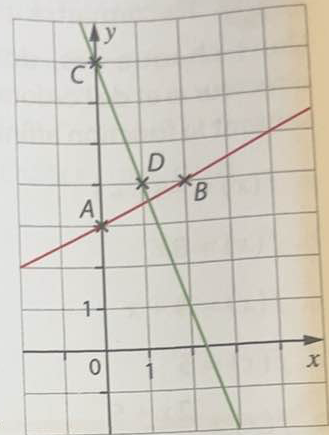
\includegraphics[scale=0.7]{1.OPT.02.07-IMG01}
\end{center}
%$$
%\begin{aligned}
%	& f(x)=\frac{1}{2} x+3 \\
%	& g(x)=-3 x+7
%\end{aligned}
%$$

\exerciceDS{}
On a représenté ci-dessous, par une droite, une fonction g. Exprimer $g(x)$ en fonction de $x$.

\begin{center}
	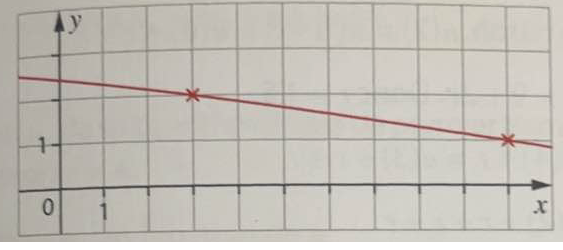
\includegraphics[scale=0.7]{1.OPT.02.07-IMG02}
\end{center}


%Cette droite représente une fonction affine.
%Le coefficient directeur est égal a $\frac{-1}{7}$.

\exerciceDS{}

La fonction $f$ est une fonction affine dont la représentation graphique passe par les points $A(-1 ; 9)$ et $B(4 ;-1)$.
\begin{enumMet}
	\item Déterminer une expression de $f(x)$ en fonction de $x$.
	\item Calculer $f(2)$.
%$$
%m=\frac{-1-9}{4-(-1)}=\frac{-10}{5}=-2, \text { donc } f(x)=-2 x+p
%$$
%$\operatorname{Or} f(-1)=9 \Leftrightarrow-2 \times(-1)+p=9$
%$$
%\Leftrightarrow p=9-2=7
%$$

%Donc $f(x)=-2 x+7$. Ainsi $f(2)=-2 \times 2+7=3$.
	\item Le point de coordonnées $(0 ; 5)$ appartient-il à la courbe représentative de $f$ ?
%$f(0)=7$, donc le point de coordonnées $(0 ; 5)$

\end{enumMet}
\exerciceDS{}

Parmi les fonctions affines définies ci-dessous, entourer celles qui sont strictement décroissantes sur $\mathbb{R}$.
\begin{multicols}{3}
\begin{enumMet}
	\item $f(x)=\dfrac{1}{4} x+1$
	\item $f(x)=-5 x+3$
	\item $f(x)=1-x$
	\item $f(x)=-9$
	\item $f(x)=-2+x$
	\item $f(x)=-6 x$
\end{enumMet}
\end{multicols}

\exerciceDS{}

Soit $g$ la fonction définie pour tout nombre réel $x$ par $g(x)=5-\dfrac{x}{2}$.
\begin{enumMet}
	\item Déterminer le sens de variation de $g$. 
%$g(x)=-\frac{1}{2} x+5$ et $-\frac{1}{2}<0$ donc $g$ est une fonction affine strictement décroissante sur $\mathbb{R}$.
	\item Comparer les valeurs de $g(72)$ et $g(79)$ sans les calculer.
%$72<79$ et $g$ est strictement décroissante sur $\mathbb{R}$, donc
%$$
%g(72)>g(79)
%$$
	\item Déterminer le signe de $g(x)$ selon les valeurs de $x$.
%$$
%g(x)=0 \Leftrightarrow 5-\frac{x}{2}=0 \Leftrightarrow \frac{x}{2}=5 \Leftrightarrow x=10
%$$
%$g$ est strictement décroissante sur $\mathbb{R}$ et s'annule en 10,
\end{enumMet}

\exerciceDS{}

Soit $f$ une fonction affine dont la représentation graphique passe par les points $A(-1 ; 4)$ et $B(4 ; 7)$.
\begin{enumMet}
	\item Déterminer une expression de $f(x)$ en fonction de $x$.
	\item Calculer $f(3)$. 

%$m=\frac{7-4}{4-(-1)}=\frac{3}{5}$ donc $f(x)=\frac{3}{5} x+p$.
%
%Or $f(-1)=4$ donc $\frac{3}{5} \times(-1)+p=4$ donc $p=4+\frac{3}{5}=\frac{23}{5}$.
%
%Donc $f(x)=\frac{3}{5} x+\frac{23}{5}$.

%Ainsi $f(3)=\frac{3}{5} \times 3+\frac{23}{5}=\frac{32}{5}$
	\item Le point $C\left(\dfrac{5}{4} ; 5,3\right)$ appartient-t-il à la courbe représentative de $f$ ?
\end{enumMet}

\end{document}

